\chapter{Previous Work}

The work of my thesis uses the universal Hasher for digital representations of music tool. This work was largely done in the Spring of 2015 as part of my undergraduate capstone supervised independent study (6.UAP). Additionally, experimental results in a related project, which focused on speeding up musical comparison by converting Python objects to C objects, provide evidence that the bottleneck in musical sequence alignment is not in the comparison step. Both subjects are described in more detail below but only to the extent necessary to understand the work of my thesis.

\section{A Modular Universal Hasher} \label{hasher}
Prior to my work on building a musical sequence aligner and fixer, I built a hasher with the specific intention that it would be able  to adapt according to different specification settings decided by the programmer. The programmer decides which kinds of \texttt{music21} stream elements, such as notes and chords, and properties, such as pitch name or duration, are relevant to their hash, and selects them to build a specific instance of a \texttt{Hasher} object. This \texttt{Hasher} instance can then be used to produce a hash from any \texttt{music21} stream. 

\subsection{Why Musical Comparison and Alignment Needs a Modular Hashing Function}
A hash function maps pieces of data of arbitrary size into data of fixed size and standard representation. If musical sequences could be discretized into elements and if these elements could be hashed, then the processes of comparison and alignment could be made deterministic and quick. 

Depending upon the problem statement that calls for a hash in the first place, this is a two step process:
\begin{enumerate}
\item discretizing a musical sequence into a list of relevant elements
\item hashing those elements  
\end{enumerate}
The details of this process can vary.  For instance, in determining the rhythmic similarity between two musical sequences, only the musical elements with durations (e.g. notes, chords, rests) in each sequence would be relevant. In hashing these elements, only properties such as duration and offset might be relevant. 

\begin{figure}[H]
\centering
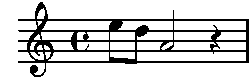
\includegraphics[scale=.7]{alg}
\caption[Rhythmic hash of a short melody]{
The hash of rhythmic features of this short melody would be \textit{NoteHash(offset=0, duration=0.5), NoteHash(offset=0.5, duration=0.5), NoteHash(offset=1.0, duration=2.0) NoteHash(offset=4, duration=1.0)}}
\end{figure}

As another example, in determining whether one piece is an approximate transposition of another, only the elements with some relation pitch (e.g. notes and chords) might be relevant.

\begin{figure}[H]
\centering
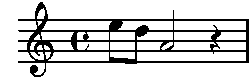
\includegraphics[scale=.7]{alg}
\caption[Melody transposition hash]{The hash of features related to transposition of this short melody would be \textit{NoteHash(intervalFromLastNote=0), NoteHash(intervalFromLastNote=-2), NoteHash(intervalFromLastNote=-5)}}
\end{figure}
Once a musical sequence is discretized and represented as a sequence of \texttt{NoteHash} objects, each individual tuple in the hash sequence can be thought of as a point in the space of all combinations of possible element properties. Then, canonical edit distance or string alignment algorithms can then be used to come up with a measure of similarity or an alignment between the two original musical sequences.

\subsection{Previous Work on Modular Hashing Functions}
The idea of extracting qualities of music specific to the needs of distance analyses and encoding that information in a lower-dimensional representation is not new. Typke in his thesis proposes what he calls a weighted point set representation of music \cite{typke}. His method of creating a weighted point set for a stream of music involves only taking melodic information (i.e. notes) and representing each discrete note as a three-tuple of (time, pitch, weight). The time component encodes information about the note's offset from the beginning. The pitch component encodes the note's pitch using the Hewlett's base-40 system (this is a numerical encoding similar to MIDI pitch but is also able to encode more information than just absolute frequency). The weight component is an assignment of how important the particular note is to the melody of the music stream." as something like "The weight component is an assignment of a numerical value to each note in the music stream, indicating the relative importance of the different notes within the melody \cite{hewlett}. 

\subsection{Overview of System}
The \texttt{Hasher} object is found in \texttt{hasher.py}. Its purpose is to identify the relevant features of relevant elements in any music stream and to represent them in a hashed format that is easy to compute with. Relevant elements here means objects such as notes, rests, chords. Relevant features here means qualities of these elements such as pitch, duration, offset. I represent these qualities in the hash as lightweight integers, floats, and strings, which makes future computations such as comparisons, and numerical operations easy and fast. 

Upon instantiation, \texttt{Hasher} does not take in any parameters. After an instance of \texttt{Hasher} is created, however, the user can set specific parameters in the \texttt{Hasher} to fit their own needs. The user must specify which relevant stream elements (notes, rests, chords) should be hashed, as well as which relevant qualities of those elements should be hashed (pitch, duration, offset, etc.). 

After the hashing parameters are set, the user calls the \texttt{hashStream} method on a stream. This method strips the stream only to the relevant elements, creates a set of hash functions based on the user's selection of relevant element qualities, and individually hashes each element with the entire set of specified hashing functions. 

The \texttt{Hasher} will create either a \texttt{NoteHash} or a \texttt{NoteHashWithReference} object for each element and add it to the end of the \texttt{FinalHash} list. Both are tuples that hold the hashed qualities of a single stream element. The only difference is that a \texttt{NoteHashWithReference} stores a reference back to the original stream element. Even though this has a lot of overhead, it is necessary if ever the original streams need to referenced for context or if they need to be changed.

The output of the entire process is a list of  \texttt{NoteHash} or \texttt{NoteHashWithReference} objects, stored in \texttt{finalHash}.

\subsubsection{Pre-Hashing: High Level Hasher Settings}
There are several system-wide high level settings that must first be set before the \texttt{hashStream} method can be called.
\begin{itemize}
\item \texttt{includeReference} - By default this is set to \texttt{False}, but if set to \texttt{True}, each element hash will be stored in a \texttt{NoteHashWithReference} object that includes a reference to the original element in its original stream. For many purposes, having this reference is not necessary and takes up extra overhead, so it is set to \texttt{False} by default.

\item \texttt{validTypes} - This is a list of the types of stream elements should be hashed. By default this is \texttt{[note.Note, note.Rest, chord.Chord]} and can be changed to be any subset of those three stream elements.
\item \texttt{stateVars} - This is a dictionary that keeps track of state between consecutive hashes. By default it doesn't contain anything, but can be programmed to contain \textit{intervalFromLastNote} and \textit{KeySignature} during the later process of preprocessing the streams and setting the appropriate hashing functions if the user-set parameters call for their use. 

\item \texttt{hashingFunctions} - This is the dictionary that stores maps which hashing functions should be used to hash which qualities. For example, if the user chose to hash notes and their MIDI pitch values, then the dictionary value for the key \textit{Pitch} would be \textit{\_hashMIDIPitchName}, the name of the function that takes a note and returns its MIDI pitch. 
\end{itemize}

        \subsubsection{Pre-Hashing: Low Level General Settings}
        These settings affect more than one of notes, rests, chords.
        
                    \begin{itemize}
                    \item \texttt{\_hashOffset} - If \texttt{True}, this will include in the hash a number that is associated with the offset of a musical element from the beginning of the stream. 
                    \item \texttt{\_hashDuration} - If \texttt{True}, this will include in the hash a number that is associated with its duration (measured in a multiplier of \texttt{duration.quarterLength}) .
                    \item \texttt{\_roundDurationAndOffset} - This is a boolean for determining whether offsets and durations should be rounded. This is useful for files (e.g. MIDI recordings without rounding) where beginnings of notes, rests, and chords may not fall exactly on the beat (e.g. beat 2.985 instead of 3).
                    \item \texttt{granularity} - A number that determines how precisely we round. If duration and offset are rounded, they will be rounded to this granularity of beat division. For example, a granularity of 32 will round notes to the nearest \nth{32} beat division and no further.
                    \end{itemize}
        
        \subsubsection{Pre-Hashing: Low Level Note Settings}
                    \begin{itemize}
                    \item \texttt{\_hashPitch} and \texttt{\_hashMIDI} - These settings determine whether the pitch of a note will be hashed, and if it is, how it will be represented. If \texttt{\_hashMIDI} is \texttt{True}, then the MIDI pitch value is hashed. Otherwise, its name representation is hashed (e.g.``C\#\#''). This setting is useful depending upon whether the user would want to differentiate between B\# and C.
                    \item \texttt{\_hashOctave} - If \texttt{True}, this includes in the hash the number octave that a note is in. This could be useful for an envelope-like following of pitches. 
                    \item \texttt{\_hashIntervalFromLastNote} - If \texttt{True}, this returns a number corresponding to the interval between the current note and the last note when applicable. This setting is a useful alternative to hashing pitch when trying to identify transpositions of pieces.
                    \item \texttt{\_hashIsAccidental} - If \texttt{True}, this will return a boolean indicating whether the pitch of the hashed element is outside of the key signature. This setting is currently not fully supported. 
                    \end{itemize}
        \subsubsection{Pre-Hashing: Low Level Chord Hashing Settings}
        Chords can be thought of as multiple notes happening at the same time. In \texttt{music21}, chords are their own type of object that can be decomposed into \texttt{note} objects. In the hashing system, chords can be hashed as chords, or by their constituent notes.
                    \begin{itemize}
                    \item \texttt{\_hashPrimeFormString} - If \texttt{True}, this includes in the hash of chord a string representation of its prime form.
                    \item \texttt{\_hashChordNormalOrderString} - If \texttt{True}, this includes in the hash of a chord a string representation of its normal order. 
                    \end{itemize}
        \subsubsection{Hashing: \texttt{hashStream}}
        Once the settings of a \texttt{Hasher} instance have been set, we can call its \texttt{hashStream} method on any stream. The following sections describe the what happens within a single \texttt{hashStreams} call. 
        \subsubsection{Hashing: Setting up \texttt{ValidTypes} and \texttt{StateVars}}
        First, the method \texttt{setupValidTypesAndStateVars} is called to set up the state variables and the valid hashing types. Recall that by default \texttt{stateVars} is empty and \texttt{validTypes} is \texttt{[note.Note, note.Rest, chord.Chord]} (of course, the user has already had the option of changing \texttt{validTypes} to contain any subset of the default types). This method checks whether the user has set either of these two settings:
        \begin{enumerate}
        \item \texttt{hashIntervalFromLastNote} - if this is set, then \texttt{IntervalFromLastNote} is added to \texttt{stateVars} to keep track of it. 
        \item \texttt{hashIsAccidental} - if this is set, then \texttt{KeySignature} is added to \texttt{stateVars} to keep track of, and \texttt{key.KeySignature} is added to the list of \texttt{validTypes} to hash. 
        \end{enumerate}
        
        \subsection{Hashing: Preprocessing the Stream}
        The stream that the \texttt{hashStream} method acts upon is stripped of all note ties in the \texttt{preprocessStream} if the \texttt{stripTies} setting is \texttt{True}. Additionally, this method returns the stream in a generator form by calling \texttt{recurse} on the stream. 
        
        \subsubsection{Hashing: Creating a List of Elements to be Hashed}
        Next the \texttt{hashStream} method builds a list of elements that are to be hashed by filtering the recursed stream of any types that are not in \texttt{validTypes}. This is stored in \texttt{finalEltsToBeHashed}.
        
        \subsubsection{Hashing: Building a Set of Hashing Functions}
        The method \texttt{setupTupleList} is called, and it sets up \texttt{tupleList}, \texttt{hashingFunctions} and \texttt{tupleClass}, all related to each other. \texttt{tupleList} is a list of all the element properties that should be hashed. \texttt{hashingFunctions} is a dictionary of which hashing function should be used for each property. \texttt{tupleClass} is a \texttt{namedtuple} that is constructed ad hoc based on which properties are to be hashed. The ad hoc construction accommodates for the fact that different \texttt{Hasher} instances will contain different things to hash. 
        
        \subsubsection{Hashing: Creating a \texttt{NoteHash} for Every Element}
        For each of the elements in \texttt{finalEltsToBeHashed}, the \texttt{Hasher} hashes its relevant properties using the hashing function listed in \texttt{hashingFunctions}. It then creates a single \texttt{NoteHash} that stores all the hashed properties.
        
        \subsubsection{Hashing: Building \texttt{finalHash}}
        If \texttt{includeReference} is set to \texttt{False}, then each new \texttt{NoteHash} object is directly added to \texttt{finalHash}. If \texttt{includeReference} is \texttt{True}, then each \texttt{NoteHash} gets replaced with a \texttt{NoteHashWithReference} object that includes a reference to the original stream element, and that gets added to \texttt{finalHash} instead.
    
\section{Low-level Object Comparison Optimizations} \label{spaceoptimizations}
Work during the fall of 2015 focused on optimizing the comparison process with variable-length data. The underlying idea was that Python objects tend to have more overhead than C objects, and if comparison and alignment algorithms were going to be doing a lot of comparisons between \texttt{NoteHash} objects produced by the Hasher, then converting these Python objects into C objects of appropriate size could save a lot of time. Here, ``appropriate size'' refers to the idea that NoteHash objects with only a few hashed properties would correspond to smaller C objects, and \texttt{NoteHash} objects with more hashed properties would correspond to larger C objects. 

A smart implementation of the most efficient method, Yeti Levenshtein, already exists in C, so my work was to cleverly convert variable-length \texttt{NoteHash} Python objects to C objects to use the Yeti Levenshtein library\cite{yeti}, which I hoped would be faster than using any Python edit distance algorithm.

I observed that the speedup we gained in converting variable-length NoteHash Python objects to C objects to use this library was a negligible cost compared to the run time of the comparison algorithm. This empirical evidence suggested that massive parallelization and speedup of the comparison process is difficult and that optimizations in alignment would be the key to significant speedup.

Thus, I concluded that musical comparison was already near the boundaries of its optimization and my work turned to focus on creating a robust alignment algorithm, which is described in the next chapter.  